\chapter{Analyse du projet}
\section{Contexte}
Le langage Extensible Markup Language ou XML est utilisé à des fins de stockage de données, et est structuré par un schéma qui lui est associé, il permet de definir la structure et le type de contenu du document, en plus de permettre de verifier la validité du document.
\paragraph{}

Généralement, les fichiers XML sont générés par un programme quelconque dans le but d'échanger des données ou de les stocker, XML faisant office de plateforme commune. Mais on peut également utiliser un éditeur de texte basique pour créer de toute pièce un document XML, avec des fonctionnalités propre à un éditeur de texte, sans fonctionnalités spécialement prévues pour XML.
\paragraph{}

C'est dans ce contexte que des solutions logicielles d'éditeur XML ont vu le jour : un éditeur de texte qui possède des fonctionnalités permettant une écriture d'un fichier XML beaucoup plus rapide et efficace, le tout avec un contrôle des erreurs.
	
\section{Analyse de l'existant}
Plusieurs solutions sont déjà proposées, certaines étant payantes et d'autres sont gratuites et open source. L'objectif est ici de fournir une solution similaire aux autres logiciels.
\paragraph{}

En se basant sur le logiciel le plus pertinent d'après les recherches autour du sujet "xml editor", le logiciel oXygen XML Editor semble être le plus présent et utilisé. C'est une solution logicielle contenant deux principaux outils : XML Developer et XML Author. Le tarif pour le package complet de XML Editor est au prix de 488\$ ou 19\$ par mois là ou chaque outil coûte à l'unité 349\$, ce qui en fait un logiciel très onéreux. L'entreprise propose cependant une version d'essai de 30 jours pour tester le logiciel. Le programme propose un nombre très important de fonctionnalités dans le but d'être utilisable à la fois par un développeur qui connaît déjà le langage et qui voudrait optimiser la saisie de fichiers XML et par un novice de XML avec un système d'assistants de création de documents.
\paragraph{}

La figure \ref{oxygen} expose par exemple une vue spéciale du document sous forme de tableur, permettant une modification beaucoup plus aisée des attributs des nœuds.

%\newpage
\vfill

\begin{figure}[H]
      \centering
      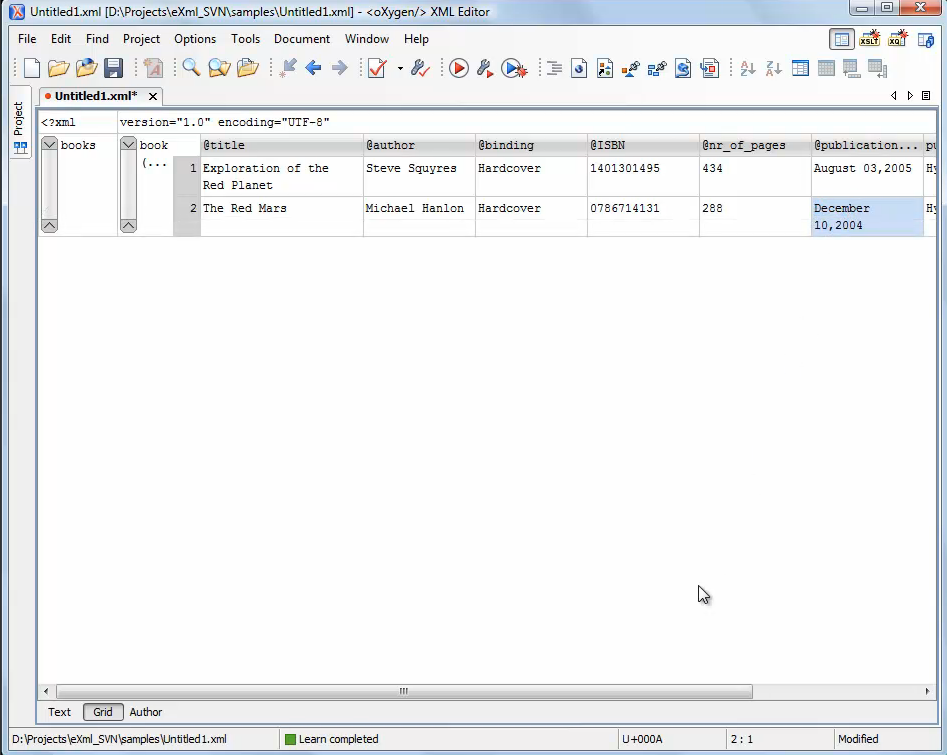
\includegraphics[scale=0.5]{images/analyse-oxygen1.png}
      \caption[Maquette d'interface]{Maquette qsdqdsqsdd'interface.}
\end{figure}


\vfill
\clearpage

\begin{figure}[h!]
\begin{minipage}[b]{\linewidth}
\centering 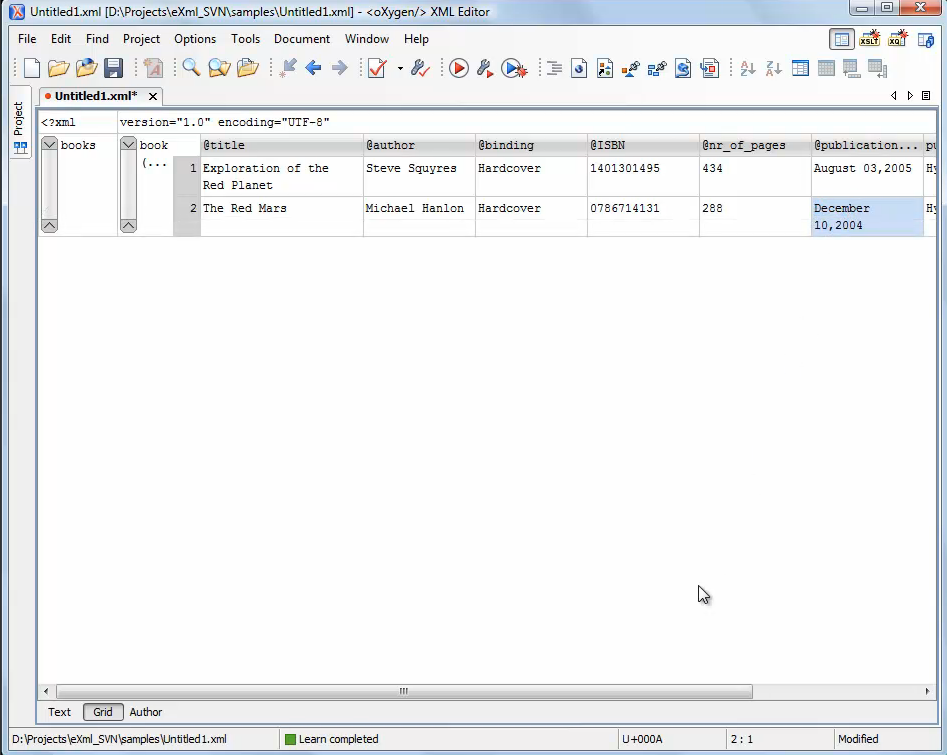
\includegraphics[scale=0.5]{images/analyse-oxygen1.png}
\caption{Exemple de vue avec Oxygen}
\label{oxygen}
\end{minipage}
\end{figure}


\section{Analyse des besoins fonctionnels}
L'objectif du projet est de développer un éditeur XML multi-vues avec différentes fonctionnalités.
\paragraph{}
Les fonctionnalités liées à un éditeur de texte simple devront être présentes : la possibilité de saisir manuellement au clavier l'intégralité du fichier, la création et la sauvegarde du fichier à manipuler ainsi que l'ouverture d'un fichier déjà existant dans le but de le modifier. La figure \ref{diagfichier} présente les différents cas d'utilisation de l'application pour ce qui est de la gestion de fichiers brute.

\begin{figure}[h!]
\begin{minipage}[b]{\linewidth}
\centering 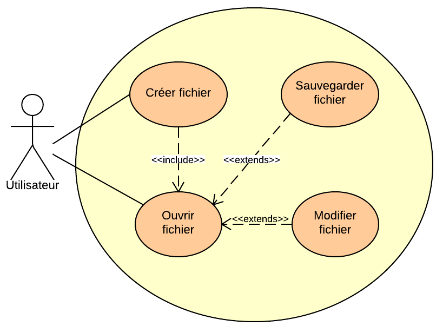
\includegraphics[scale=0.5]{images/analyse-diag-fichier.png}
\caption{Diagramme des cas d'utilisation côté gestion des fichiers}
\label{diagfichier}
\end{minipage}
\end{figure}

\paragraph{}
Des fonctionnalités d'éditeur de texte avancées seront aussi présentes : coloration syntaxique et indentation automatique du code permettant ainsi une lisibilité claire des fichiers manipulés et une autocomplétion du code écrit permettant un gain de temps au cours de la frappe.
\paragraph{}
Pour finir, l'éditeur proposera des fonctionnalités spécifiques au langage XML : validation syntaxique du fichier, vue arborescente du fichier XML avec possibilité de modification des données via cette vue et ajout d'un schéma sur lequel la validation se basera. Les différentes actions réalisables via la vue arborescente sont exposées dans la figure \ref{diagarbo}. Les actions liées à l'éditeur de texte même et à la vérification syntaxique sont elles décrites sur la figure \ref{diagediteur}.

\begin{figure}[h!]
\begin{minipage}[b]{\linewidth}
\centering 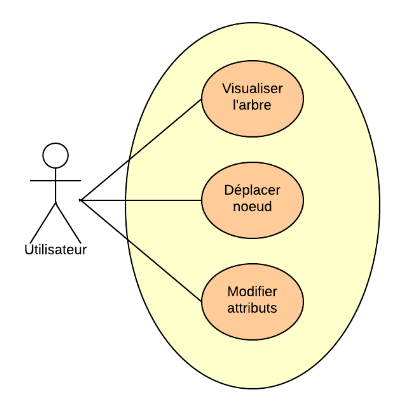
\includegraphics[scale=0.5]{images/analyse-diag-arbo.png}
\caption{Diagramme des cas d'utilisation de la vue arborescente}
\label{diagarbo}
\end{minipage}
\end{figure}

\begin{figure}[h!]
\begin{minipage}[b]{\linewidth}
\centering 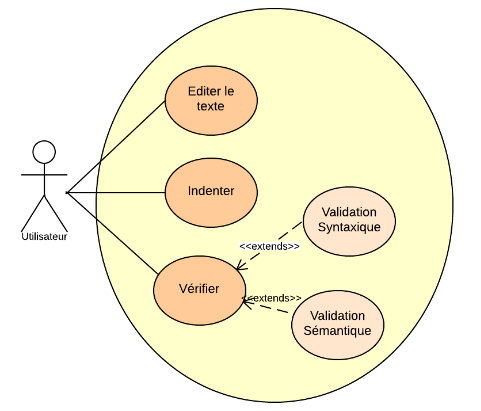
\includegraphics[scale=0.5]{images/analyse-diag-editeur.png}
\caption{Diagramme des cas d'utilisation de l'éditeur de texte}
\label{diagediteur}
\end{minipage}
\end{figure}

\paragraph{}	
La figure \ref{maquette_interface} expose la maquette d'interface de l'éditeur avec chacune des parties annoncées : à gauche la vue arborescente affichant chaque nœud de l'arbre formé par les données, à droite l'éditeur de texte avec toutes ses fonctionnalités associées et en haut la barre d'outils avec la gestion de fichiers (nouveau fichier, ouvrir, sauvegarder) ainsi que la gestion du schéma.

\begin{figure}[h!]
\begin{minipage}[b]{\linewidth}
\centering 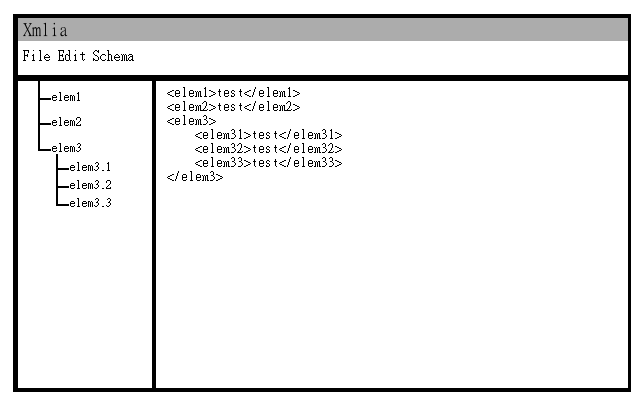
\includegraphics[scale=0.5]{images/analyse-maquette.png}
\caption{Maquette d'interface}
\label{maquette_interface}
\end{minipage}
\end{figure}
	
\section{Analyse des besoins non fonctionnels}
\subsection{Spécifications techniques}
Le programme devra permettre de créer des fichiers XML structurés avec un respect des normes de balisage et, s'il est défini, du schéma de données. De plus, les données saisies ou modifiées à l'aide de l'éditeur doivent rester exploitables, sans corruption du fichier original. Pour terminer, l'éditeur aura à répondre dans des durées acceptables et de manière stable, dans la mesure où la taille et la complexité des données restent raisonnables.
		
\subsection{Contraintes ergonomiques}
Le logiciel devra être suffisamment simple pour qu'un utilisateur connaissant déjà le fonctionnement du XML puisse l'utiliser sans être bloqué par une courbe d'apprentissage trop élevée. On utilisera pour cela des icônes claires et des textes explicatifs.
\paragraph{}
Un utilisateur avancé pourra augmenter sa productivité en utilisant les raccourcis clavier disponibles et pourra gagner de temps en réduisant les transitions souris/clavier.
